\documentclass{beamer}

% Packages

% Sets

% Formal statements


\title{Diseño y análisis de algoritmos \\ ISIS1105}
\author{Daniel R. Barrero R.}
\institute{Universidad de los Andes}

\begin{document}
\frame{\titlepage}

%

\begin{frame}{LRRs - Homogenization trick}
	\begin{thm}[2]\label{ht}
		If the initial value problem
		\begin{displaymath}(4)
			\begin{cases}
				t(0)= v_0, \cdots, t(k-1)= v_{k-1}\\
				t(n) + \sum_{i= 1}^k b_it(n-i)= q,\ n \geq k
			\end{cases}
		\end{displaymath}
		is such that $q = c^np(n)$, where $c$ is a positive constant and
		$p(n)$ is a polynomial of degree $d$, then it is equivalent to a
		homogeneous problem of degree $k+d+1$ with characteristic equation
		\begin{equation*}
			E(x)(x-c)^{d+1} = 0
		\end{equation*}
		where $E(x) = 0$ is the characteristic equation of the recurrence
		in (4).
	\end{thm}
\end{frame}

%% Divide and conquer
\begin{frame}{Divide and conquer}
	\centering
	
\includegraphics[width=0.3\textwidth]{strategist.png}
	
	\bigskip
	``\emph{Unity is strength. Divide your enemy, and conquer them.}''
\end{frame}

%

\begin{frame}{D \& C - fast exponentiation}
	Consider the following algorithm
	
	\lstinputlisting[language=Java, firstline=8, lastline=18]{Aula06.java}
	
	Let $t(n)$ denote the number of multiplications \texttt{'*'}. It defines the
	initial value problem
	\[
		\begin{cases}
			t(0)= 0\\
			t(n)= t(n/2) + 1,\ n > 0\ \text{even}\\
			t(n)= t(n-1) + 1,\ n > 0\ \text{odd}.
		\end{cases}
	\]
\end{frame}

%

\begin{frame}{D \& C - fast exponentiation}
	To compute its time complexity, notice that
	\[
		\lfloor n/2 \rfloor =
		\begin{cases}
			n/2,\ n \text{ even}\\
			(n-1)/2,\ n \text{ odd}.
		\end{cases}
	\]
	Therefore, if $n$ is odd
	\[
		\begin{array}{c}
			t(n) = \left( t\left( \frac{n-1}{2} \right) + 1 \right) + 1\\
			= t(\lfloor n/2 \rfloor) + 2.
		\end{array}
	\]
	Then $t(n) \in O(\tau(n))$ where
	\[
		\begin{cases}
			\tau(0)= 0\\
			\tau(n)= \tau(\lfloor n/2 \rfloor) + 2,\ n > 0.
		\end{cases}
	\]
\end{frame}

%

\begin{frame}{D \& C - fast exponentiation}
	We apply the change of variable $n= 2^m$ and let $T(m)= \tau(2^m)$. We
	obtain the i.v.p.
	\[
		\begin{cases}
			T(0)= 2\\
			T(m)= T(m-1) + 2,\ m > 0.
		\end{cases}
	\]
	We apply the homogenization trick. If $m > 1$ then
	\[
		\begin{array}{c}
			T(m) - T(m-1) = 2\\
			T(m-1) - T(m-2) = 2.
		\end{array}
	\]
	Then a closed formula for $T(m)$ is obtained by solving the homogeneous i.v.p.
	\[
		\begin{cases}
			T(0)= 2,\ T(1) = 4\\
			T(m) - 2T(m-1) + T(m-2)= 0,\ m > 1.
		\end{cases}
	\]
\end{frame}

%

\begin{frame}{D \& C - fast exponentiation}
	The characteristic equation is $(x - 1)^2= 0$, so the solution is
	\[
		T(m) = u1^m + vm1^m
	\]
	where the constants $u$ and $v$ are such that
	\[
		\begin{cases}
			u = 2\\
			u + v = 4.
		\end{cases}
	\]
	This gives $T(m) = 2 + 2m$. Since $m = \log n$, we obtain
	\[
		\tau(n) = 2 + 2\log n
	\]
	and we conclude $t(n) \in O(\log n)$.
\end{frame}

%

\begin{frame}{D \& C - master theorem}
	Let $t(n)$ be such that
	\[
		t(n) \leq at(n/b) + cn^k
	\]
	for $c \in \Rpos$, $a \in \Zpos$, $b \in \Zpos$, $k \in \NN$ and $n$ a
	large enough power of $b$. Then
	\[
		t(n) \in
		\begin{cases}
			O(n^k)\ \ \text{if}\ a < b^k\\
			O(n^k\log n)\ \ \text{if}\ a = b^k\\
			O(n^{\log_b a})\ \ \text{if}\ a > b^k.
		\end{cases}
	\]
\end{frame}

%

\begin{frame}{D \& C - Proof of master theorem}
	The essential step in the proof of the master theorem is equivalent to
	computing the time complexity of the following recurrence. Let $a \in \Zpos,
	b \in \ZZ^{\geq 2},\ c \in \Rpos$.
	\[
		\begin{cases}\label{mtr} % Master theorem recurrence
			t(1)= v_0\\
			t(n)= at(\lceil n/b \rceil) + cn^k,\ n > 1.
		\end{cases}
	\]
	After the change of variable $T(m)= t(b^m)$, it becomes the linear initial
	value problem
	\[
		\begin{cases}\label{mtl} % Master theorem linear
			T(0)= v_0\\
			T(m)= aT(m-1) + c(b^k)^m,\ m > 0.
		\end{cases}
	\]
\end{frame}

%

\begin{frame}{D \& C - Proof of master theorem}
	To apply the homogenization trick, we see that for $m > 1$ we have 
	\[
		\begin{cases}
			T(m) - aT(m-1) = c(b^k)^m\\
			b^kT(m-1) - ab^kT(m-2) = c(b^k)^m
		\end{cases}
	\]
	Subtracting these equations and computing $T(1)$, we obtain the homogeneous
	initial value problem
	\[
		\begin{cases}
			T(0)= v_0,\ T(1)= av_0 + cb^k\\
			T(m) - (a + b^k)T(m-1) + ab^kT(m-2)= 0,\ m > 1.
		\end{cases}
	\]
\end{frame}

%

\begin{frame}{D \& C - Proof of master theorem}
	Its characteristic equation is $(x - a)(x - b^k)= 0$, so that the solution
	is of the form
	\[
		T(m) = ua^m + v(b^k)^m
	\]
	for some constants $u$ and $v$, unless $a = b^k$, in which case
	\[
		T(m) = u(b^k)^m + vm(b^k)^m.
	\]
	The result then follows from noticing that $a^m = n^{\log_b a}$ and
	$(b^k)^m = n^k$, and by considering the possible values of the limit
	\[
		\lim_{m \to \infty} \frac{a^m}{(b^k)^m}.
	\]
\end{frame}

%% Dynamic programming
\begin{frame}{Dynamic programming (DP)}
	\centering
	
\includegraphics[width=0.4\textwidth]{tyler.png}

	``\emph{Sometimes sub-problems overlap, believe me. In that case, we keep
		track of the smaller solutions in a table. That's what we call
		dynamic programming.}''
\end{frame}

%

% Binomial coefficients
\begin{frame}{DP - Binomial coefficients}
	\centering
	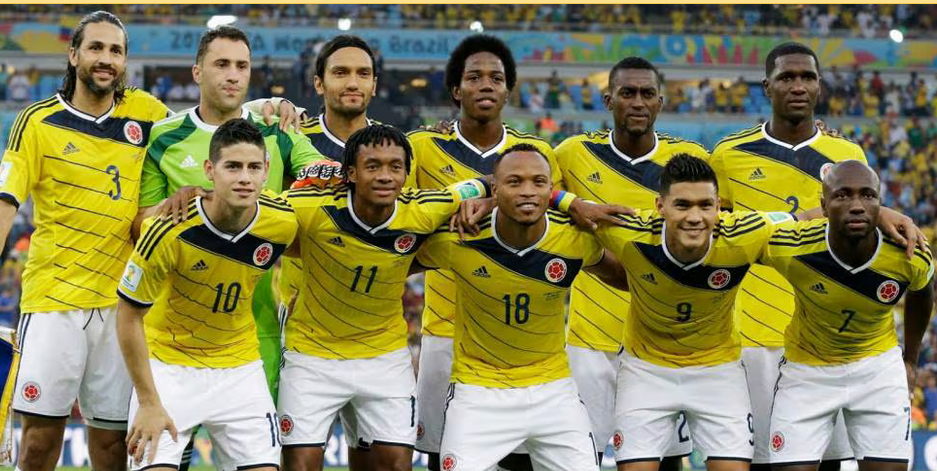
\includegraphics[width=0.6\textwidth]{sele2014.png}
	\hspace{0.5cm}
	$\longleftarrow$
	\hspace{0.5cm}
	
\includegraphics[width=0.15\textwidth]{lucho.png}
\end{frame}

%

% No teams
\begin{frame}{DP - Binomial coefficients}
	\centering
	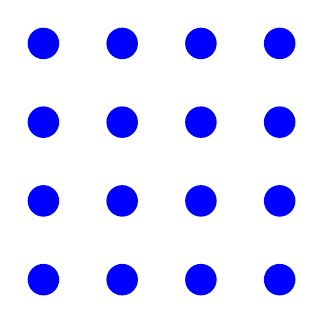
\begin{tikzpicture}
		\node at (1,1) [circle, inner sep=0, minimum size=4mm, fill=blue] {};
		\node at (1,2) [circle, inner sep=0, minimum size=4mm, fill=blue] {};
		\node at (1,3) [circle, inner sep=0, minimum size=4mm, fill=blue] {};
		\node at (1,4) [circle, inner sep=0, minimum size=4mm, fill=blue] {};
		\node at (2,1) [circle, inner sep=0, minimum size=4mm, fill=blue] {};
		\node at (2,2) [circle, inner sep=0, minimum size=4mm, fill=blue] {};
		\node at (2,3) [circle, inner sep=0, minimum size=4mm, fill=blue] {};
		\node at (2,4) [circle, inner sep=0, minimum size=4mm, fill=blue] {};
		\node at (3,1) [circle, inner sep=0, minimum size=4mm, fill=blue] {};
		\node at (3,2) [circle, inner sep=0, minimum size=4mm, fill=blue] {};
		\node at (3,3) [circle, inner sep=0, minimum size=4mm, fill=blue] {};
		\node at (3,4) [circle, inner sep=0, minimum size=4mm, fill=blue] {};
		\node at (4,1) [circle, inner sep=0, minimum size=4mm, fill=blue] {};
		\node at (4,2) [circle, inner sep=0, minimum size=4mm, fill=blue] {};
		\node at (4,3) [circle, inner sep=0, minimum size=4mm, fill=blue] {};
		\node at (4,4) [circle, inner sep=0, minimum size=4mm, fill=blue] {};
	\end{tikzpicture}
	\hspace{1cm}
	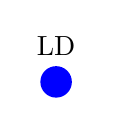
\begin{tikzpicture}
		\node at (1,1) [circle, inner sep=0, minimum size=4mm, fill=blue,
			label=above:LD] {};
	\end{tikzpicture}

	\medskip
	\[
		\ 
	\]
\end{frame}

%

% Without new
\begin{frame}{DP - Binomial coefficients}
	\centering
	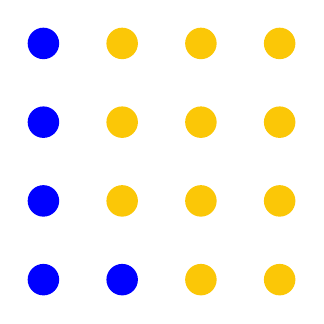
\begin{tikzpicture}
		\colorlet{syellow}{yellow!60!orange}
		\node at (1,1) [circle, inner sep=0, minimum size=4mm, fill=blue] {};
		\node at (1,2) [circle, inner sep=0, minimum size=4mm, fill=blue] {};
		\node at (1,3) [circle, inner sep=0, minimum size=4mm, fill=blue] {};
		\node at (1,4) [circle, inner sep=0, minimum size=4mm, fill=blue] {};
		\node at (2,1) [circle, inner sep=0, minimum size=4mm, fill=blue] {};
		\node at (2,2) [circle, inner sep=0, minimum size=4mm, fill=syellow] {};
		\node at (2,3) [circle, inner sep=0, minimum size=4mm, fill=syellow] {};
		\node at (2,4) [circle, inner sep=0, minimum size=4mm, fill=syellow] {};
		\node at (3,1) [circle, inner sep=0, minimum size=4mm, fill=syellow] {};
		\node at (3,2) [circle, inner sep=0, minimum size=4mm, fill=syellow] {};
		\node at (3,3) [circle, inner sep=0, minimum size=4mm, fill=syellow] {};
		\node at (3,4) [circle, inner sep=0, minimum size=4mm, fill=syellow] {};
		\node at (4,1) [circle, inner sep=0, minimum size=4mm, fill=syellow] {};
		\node at (4,2) [circle, inner sep=0, minimum size=4mm, fill=syellow] {};
		\node at (4,3) [circle, inner sep=0, minimum size=4mm, fill=syellow] {};
		\node at (4,4) [circle, inner sep=0, minimum size=4mm, fill=syellow] {};
	\end{tikzpicture}
	\hspace{1cm}
	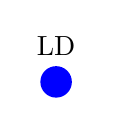
\begin{tikzpicture}
		\node at (1,1) [circle, inner sep=0, minimum size=4mm, fill=blue,
			label=above:LD] {};
	\end{tikzpicture}

	\[
		\binom{17}{11} = \binom{16}{11} + \binom{16}{10}
	\]
\end{frame}

%

% With new
\begin{frame}{DP - Binomial coefficients}
	\centering
	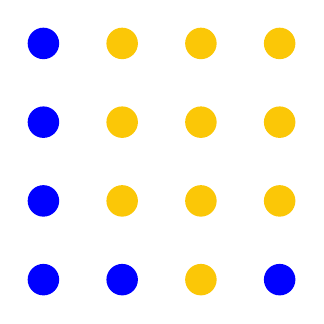
\begin{tikzpicture}
		\colorlet{syellow}{yellow!60!orange}
		\node at (1,1) [circle, inner sep=0, minimum size=4mm, fill=blue] {};
		\node at (1,2) [circle, inner sep=0, minimum size=4mm, fill=blue] {};
		\node at (1,3) [circle, inner sep=0, minimum size=4mm, fill=blue] {};
		\node at (1,4) [circle, inner sep=0, minimum size=4mm, fill=blue] {};
		\node at (2,1) [circle, inner sep=0, minimum size=4mm, fill=blue] {};
		\node at (2,2) [circle, inner sep=0, minimum size=4mm, fill=syellow] {};
		\node at (2,3) [circle, inner sep=0, minimum size=4mm, fill=syellow] {};
		\node at (2,4) [circle, inner sep=0, minimum size=4mm, fill=syellow] {};
		\node at (3,1) [circle, inner sep=0, minimum size=4mm, fill=syellow] {};
		\node at (3,2) [circle, inner sep=0, minimum size=4mm, fill=syellow] {};
		\node at (3,3) [circle, inner sep=0, minimum size=4mm, fill=syellow] {};
		\node at (3,4) [circle, inner sep=0, minimum size=4mm, fill=syellow] {};
		\node at (4,1) [circle, inner sep=0, minimum size=4mm, fill=blue] {};
		\node at (4,2) [circle, inner sep=0, minimum size=4mm, fill=syellow] {};
		\node at (4,3) [circle, inner sep=0, minimum size=4mm, fill=syellow] {};
		\node at (4,4) [circle, inner sep=0, minimum size=4mm, fill=syellow] {};
	\end{tikzpicture}
	\hspace{1cm}
	
\begin{tikzpicture}
		\colorlet{syellow}{yellow!60!orange}
		\node at (1,1) [circle, inner sep=0, minimum size=4mm, fill=syellow,
			label=above:LD] {};
	\end{tikzpicture}

	\[
		\binom{17}{11} = \binom{16}{11} + \binom{16}{10}
	\]
\end{frame}

%

% bbc - statement
\begin{frame}{DP - Binomial coefficients}
	\begin{thm}[Pascal's identity]\label{pascid}
		Let $n, k \in \NN$ be such that $0 < k < n$. Then
		\[
			\binom{n}{k} = \binom{n-1}{k} + \binom{n-1}{k-1}.
		\]
	\end{thm}

	We could then implement the following naive algorithm:
	\lstinputlisting[language=Java, firstline=24, lastline=32]{Aula07.java}
\end{frame}

%

% bbc - complexity
\begin{frame}{DP - Binomial coefficients}
	But how bad is it?
	\begin{defn}[Omega notation]
		Let $f : \NN \to \Rpos$. We define
		\[
			\Omega(f)= \{\tau : \NN \to \Rpos | f \in O(\tau)\}.
		\]
	\end{defn}
	Informally, we could say that $\Omega(f)$ consists of the functions
	``Worse than $f$''.

	\bigskip
	To analyse the complexity of \texttt{badBc}, let us count the number of
	additions given by the operator \texttt{'+'}.
\end{frame}

%

\begin{frame}{DP - Binomial coefficients}
	Let $S(n,k)$ be the number of additions \texttt{'+'} required to compute
	\texttt{badBc(n,k)}. Then
	\[
		\begin{cases}
			S(n,k) = 0,\ k = 0 \lor k = n\\
			S(n,k) = S(n-1,k) + S(n-1,k-1),\ 0 < k < n.
		\end{cases}
	\]
	It follows from a routine proof by induction that
		\[
			S(n,k) = \binom{n}{k} - 1.
		\] 
\end{frame}

%

\begin{frame}{DP - Binomial coefficients}
	We know that a set with $k$ elements has $2^k$ subsets. Also, a counting
	argument gives
	\[
		\binom{n}{k} = \sum_{j= 0}^k \binom{k}{j} \binom{n-k}{k-j}.
	\]
	Since $\binom{n-k}{k-j} \geq 1$, we obtain
	\[
		\binom{n}{k} - 1 \geq 2^k - 1.
	\]
	Thus, we may say that the complexity of \texttt{badBc} given by $S(n,k)$ is
	\emph{worse than exponential}. For instance, if we take $k= \lfloor n/2
	\rfloor$ then 
	\[
		t_{\texttt{badBc}} \in \Omega(\sqrt{2}^n).
	\]
\end{frame}

%

\begin{frame}{DP - Binomial coefficients}
	Hower, if we can manage to ``just write down Pascal's triangle'', the
	computation becomes much cheaper.
	\[
		\begin{array}{cccccc}
			1 & & & & & \\
			1 & 1 & & & & \\ 
			1 & 2 & 1 & & & \\ 
			1 & 3 & 3 & 1 & & \\ 
			1 & 4 & 6 & 4 & 1 & \\ 
			1 & 5 & 10 & 10 & 5 & 1\\
			 & \cdots & & & & 
		\end{array}
	\]
	We just keep an array of length $k$ and update it at each step.
\end{frame}

%

\begin{frame}{DP - Binomial coefficients}
	\lstinputlisting[language=Java, firstline=8, lastline=22]{Aula07.java}
	\emph{What are the time and space complexities of} \texttt{goodBc}?
\end{frame}

% World series
\begin{frame}{DP - Mario Kart world cup finals}
	\centering
	
\includegraphics[width=0.3\textwidth]{feid.png}
	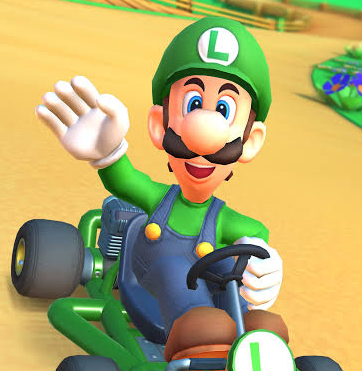
\includegraphics[width=0.3\textwidth]{luigi.png}

	VS.

	\medskip
	
\includegraphics[width=0.3\textwidth]{karolg.png}
	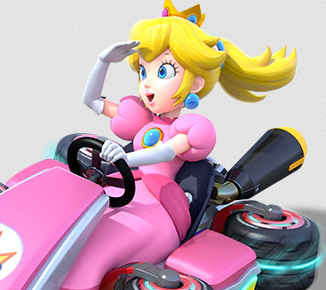
\includegraphics[width=0.3\textwidth]{peach.png}
\end{frame}

%

\begin{frame}{DP - Mario Kart}
	Two players, A and B, compete to be the first to win $n$ races.

	\bigskip
	We assume the results of the races are independent, so that the probability
	of A winning a single race is always $p \in (0,1)$ and  that of B is always
	$q = 1-p$.

	\bigskip
	Let $P(i,j)$ denote the probability that A will be the overall winner, given
	that it must win $i$ more races and B must win $j$ more races. Then

	\[
		\begin{cases}
			P(0,j) = 1\\
			P(i,0) = 0\\ 
			P(i,j) = pP(i-1,j) + qP(i,j-1),\ i > 0 \land j > 0.
		\end{cases}
	\]
\end{frame}

%

\begin{frame}{DP - Mario Kart}
	We then use the recurrence to implement the naive algoritm:
	\lstinputlisting[language=Java, firstline=61, lastline=70]{Aula07.java}
	How bad is it?
\end{frame}

%

\begin{frame}{DP - Mario Kart}
	We reformulate the problem by letting $P'(m,j)$ denote the probability that
	A will win given that B must win $j$ more races and A must win $m-j$ more
	races. Namely, $m = i+j$ in the previous formulation. Then $P'$ satisfies
	the recurrence
	\[
		\begin{cases}
			P'(j,j)= 1,\ P'(m,0)= 1\\
			P'(m,j) = pP'(m-1,j) + qP'(m-1,j-1),\ j > 0 \land m-j > 0.
		\end{cases}
	\]
	It follows that
	\[
		O(t_{\texttt{badMarioKart}}) = O(t_{\texttt{badBc}}).
	\]
	In particular, to compute the value of interest $P(n,n) = P'(2n,n)$ we have
	\[
		t_{\texttt{badMarioKart}} \in \Omega(2^n).
	\]
\end{frame}

%

\begin{frame}{DP - Mario Kart}
	However, if we record the values of $P(i,j)$ from smallest to largest values
	of the indices (a.k.a. \emph{bottom-up solving}), time complexity becomes
	quadratic:
	\lstinputlisting[language=Java, firstline=40, lastline=45]{Aula07.java}
\end{frame} % code break

%

\begin{frame}{DP - Mario Kart} % code continuation
	\lstinputlisting[language=Java, firstline=46, lastline=59]{Aula07.java}
\end{frame}

%

\begin{frame}{Dynamic programming}
	\centering
	
\includegraphics[width=0.6\textwidth]{tyler2.png}

	\bigskip
	``\emph{So you see, we trade time with space complexity. Happy now?}\,''
\end{frame}
\end{document}
